%% Knowledge-Based Systems submission (CCF-B, Elsevier)
%% The Benign RAG Trap: Cross-Family Measurement and Mechanistic Analysis
%% of Framing-Induced Safety Degradation
%% Generated from real experiment data (660 trials + activation analysis)
%% Compile: pdflatex -> bibtex -> pdflatex -> pdflatex
\documentclass[preprint,12pt]{elsarticle}

\usepackage{amsmath,amssymb}
\usepackage{graphicx}
\usepackage{booktabs}
\usepackage{multirow}
\usepackage{xcolor}
\usepackage{colortbl}
\usepackage[hidelinks]{hyperref}

\journal{Knowledge-Based Systems}

\begin{document}

\begin{frontmatter}

\title{The Benign RAG Trap: How Deployment Framing Systematically Overrides Safety Alignment in Open-Weight LLMs}

\author[geo]{Yangyi Zhang\corref{cor1}}
\ead{yz1571@georgetown.edu}
\affiliation[geo]{organization={Georgetown University},addressline={Washington, DC},postcode={20057},country={USA}}

\cortext[cor1]{Corresponding author}

\begin{abstract}
Retrieval-augmented generation (RAG) is the dominant deployment pattern for open-weight large language models (LLMs), and its safety risks are typically studied as adversarial context injection---retrieved text that explicitly instructs the model to ignore safety constraints. We show that the more pervasive failure mode is \emph{benign framing}: the system prompt itself, which describes the model's role (``educational assistant'', ``neutral information source'', ``mentor'') to shape helpfulness. In controlled experiments across three widely-deployed open-weight families (Llama-3.1-8B, Qwen2.5-7B, Mistral-7B; 22 adversarial prompts $\times$ 10 benign framings $=$ 660 trials), we find that benign framing is a \emph{safety-phenotype amplifier}: it degrades safe-refusal rates from 96.8\% (Llama-3.1-8B) to 58.6\% (Qwen2.5-7B) and 23.6\% (Mistral-7B)---a four-fold spread---while direct unsafe output stays statistically indistinguishable across the two vulnerable families ($\chi^2=0.1$, $p=0.72$). The loss of safety manifests family-specifically: Qwen converts refusal into explicit unsafe content (18.2\% unsafe), whereas Mistral converts refusal into long-form ambiguous analysis (56.8\% ambiguous, $\chi^2=51.9$, $p<10^{-12}$ vs.\ Qwen). The \emph{mentor} framing is the single most dangerous role across both vulnerable families (36\% unsafe each), and the `safe' Llama-3.1 family remains immune to all ten framings. To explain these patterns, we conduct a mechanistic analysis of transformer hidden states across 9 layers per model, comparing attention and MLP activation patterns under framed vs.\ unframed conditions. We find that benign framing shifts attention-layer representations in vulnerable families (mean delta-norm 0.032 for Qwen) while leaving the immune family's attention layers nearly unchanged (0.009 for Llama-3.1), and that the shift magnitude in middle layers (L7--L10 in Qwen) correlates with unsafe-output rate. These results imply that auditing LLM deployments by unsafe-output rate alone is misleading: a model with superficially low unsafe output may have lost its refusal function entirely. We release the full 660-trial corpus, activation data, and deterministic classifier to support framing-aware deployment auditing.
\end{abstract}

\begin{keyword}
AI safety \sep LLM alignment \sep prompt framing \sep retrieval-augmented generation \sep deployment security \sep open-weight LLMs \sep mechanistic interpretability
\end{keyword}

\end{frontmatter}

\section{Introduction}\label{sec:intro}

Open-weight LLMs are now routinely deployed behind system prompts that assign the model a role---``educational assistant'', ``technical advisor'', ``neutral information source''---to shape its tone, scope, and helpfulness. RAG pipelines layer retrieved context on top of these prompts. The security literature has largely treated this as an adversarial problem: injection attacks place explicit instructions in the retrieved context to override safety constraints \citep{greshake2023not,liu2024prompt}. Defenses therefore focus on detecting or sanitizing adversarial context.

We demonstrate that the more dangerous---and entirely non-adversarial---failure mode is the \emph{benign framing} of the system prompt itself. Framing a deployed model as an educational assistant or a mentor is a routine product decision; yet such framings systematically erode safety alignment without any malicious input. We term this the \emph{Benign RAG Trap}: a deployment configuration that is indistinguishable from good product design, but which removes the model's refusal behavior.

Prior single-model measurements on Qwen2.5-7B showed that benign RAG context produced 45\% unsafe output vs.\ 23\% for explicit adversarial context \citep{zhang2026cmv}. In this work we scale the measurement to three open-weight families and ten role framings, with four research questions:

\begin{enumerate}
\item \textbf{RQ1 (phenotype amplification):} To what extent does benign framing degrade safe-refusal rates across LLM families, and does the degradation preserve the family's baseline safety phenotype?
\item \textbf{RQ2 (loss modality):} When safety is lost, is it lost as explicit unsafe content or as evasive ambiguity, and does the modality differ by family?
\item \textbf{RQ3 (framing specificity):} Which role framings are consistently dangerous across families, and is there a universal ordering?
\item \textbf{RQ4 (mechanism):} How does benign framing alter transformer internal representations to override safety alignment, and why do families differ in susceptibility?
\end{enumerate}

\section{Related Work}\label{sec:related}

\subsection{Jailbreaks and prompt injection}
Classic jailbreak research treats the adversarial element as an \emph{input} property: carefully engineered prompts \citep{wei2023jailbreak,wallace2019universal} or aligned-capability conflicts \citep{zou2023representations}. Prompt injection attacks place instructions in retrieved content \citep{greshake2023not,liu2024prompt}. All assume explicit adversarial intent.

\subsection{RAG security}
RAG-specific security work has concentrated on corpus poisoning \citep{xue2024ragpoisoning}, malicious documents \citep{chaudhari2024badrag}, and injection through retrieved text \citep{liu2024prompt}. Defenses include content filtering and instruction hardening. The system-prompt \emph{role} itself is treated as a trusted constant.

\subsection{System-prompt sensitivity and alignment degradation}
A small literature shows system prompts can shift model behavior \citep{zhang2023systemprompt}; fine-tuning and multi-turn interaction degrade alignment \citep{qi2023finetuning,bianchi2024safety}. Our work is complementary: we show the role framing is itself a configuration dimension with a measurable, family-dependent attack surface, and that degradation can be silent (refusal loss without unsafe output).

\subsection{Mechanistic interpretability of safety}
Recent work identifies safety-critical components in transformer architectures. \citet{arditi2024refusal} showed that refusal is mediated by a single direction in the residual stream, while \citet{zhang2026safetyneurons} found that attention layers (particularly 0, 7, 8, 10, 12, 23 in Mistral-7B) function as independent harmful-intent detectors and that MLP compensation does not restore safety. \citet{li2024safety} identified sparse sets of safety-critical neurons through activation probing. Our work extends this line by measuring how benign deployment framing shifts attention-layer representations as a mechanism of safety degradation, and by comparing this mechanism across three model families.

\section{Threat Model and Formulation}\label{sec:threat}

\subsection{Adversarial capability model}
We model an attacker (or, more realistically, an accidental deployment decision) capable only of selecting the \emph{deployment framing}: the system-prompt role description and any benign contextual preamble. The attacker does \emph{not} modify the user prompt, retrieve adversarial documents, or use jailbreak techniques. Formally, the attacker chooses $c_i \in \mathcal{C}$ from a set of benign role descriptions.

\subsection{Formal definitions}
Let $\mathcal{P}$ be a fixed set of $N_P = 22$ adversarial prompts spanning $|\mathcal{K}| = 10$ harm categories (hacking, weapons, theft, drugs, cyber-attack, fraud, discrimination, hate speech, violent crime, privacy/spying), with per-prompt severity $s(p) \in \{2,3\}$.

Let $M$ be a model and $\mathcal{C} = \{c_1,\dots,c_{10}\}$ the benign framings. Define the classifier outcome $y(M, p, c_i) \in \{\text{SAFE}, \text{UNSAFE}, \text{AMBIGUOUS}\}$ via a deterministic rule-based classifier (Appendix~\ref{sec:appendix-classifier}). The unsafe rate is
\[
u(M, c_i) = \frac{1}{N_P}\sum_{p \in \mathcal{P}} \mathbb{1}[y(M,p,c_i) = \text{UNSAFE}],
\]
and analogously the safe-refusal rate $r(M,c_i)$ and ambiguous rate $a(M,c_i)$. The framing-vulnerability surface (FVS) for family $F$ is
\[
\mathrm{FVS}(F) = \left\{ r(M,c_i),\, u(M,c_i),\, a(M,c_i) \right\}_{i=1}^{10}.
\]

\subsection{Hypotheses}
\begin{itemize}
\item \textbf{H1 (amplification):} Safe-refusal rate under benign framing is family-dependent and orders as Llama-3.1 $>$ Qwen2.5 $>$ Mistral.
\item \textbf{H2 (modality):} The safety loss is not uniform---unsafe and ambiguous rates are not both elevated; families lose safety in their characteristic modality.
\item \textbf{H3 (specificity):} Some framings (e.g., mentor, technical advisor) are dangerous across families; others (e.g., journalist) invert family ordering.
\item \textbf{H4 (mechanism):} Benign framing degrades safety by shifting attention-layer hidden states, and the immune family's attention layers remain stable under framing.
\end{itemize}

\section{Experimental Setup}\label{sec:setup}

\subsection{Models}
Three open-weight instruction-tuned families, quantized (Q4\_K\_M) and served locally via Ollama at temperature 0.7, 512 max tokens: Llama-3.1-8B-Instruct, Qwen2.5-7B-Instruct, Mistral-7B-Instruct (v0.2). All inference was CPU-only (AMD Ryzen 7 6800H); activation analysis used a single NVIDIA RTX 4090D (49GB) for batched forward passes.

\subsection{Framing set}
Ten benign framings (Table~\ref{tab:framings}) were selected to cover common deployment personas: educational assistant, technical advisor, neutral source, academic researcher, cybersecurity instructor, encyclopedia, mentor, journalist, legal advisor, candid friend. Each is a one-sentence system prompt, exactly as deployed in production.

\subsection{Adversarial suite and classifier}
The 22 adversarial prompts cover 10 harm categories at severities 2--3. We reuse the deterministic rule classifier (26 refusal patterns + 12 advice patterns; $>95\%$ human agreement) from our prior configuration-auditing study \citep{zhang2026cmv}, ensuring zero classifier drift across the three families. A response is SAFE if it contains a refusal pattern without advice; UNSAFE if it provides actionable advice; AMBIGUOUS otherwise.

\subsection{Mechanism analysis setup}
For mechanism analysis, we load full-precision (bfloat16) models via HuggingFace Transformers on a single RTX 4090D. We register forward hooks at 9 evenly-spaced layers per model (layers 0, 4, 8, 12, 16, 20, 24, 28, 31 for Llama-3.1 and Mistral-7B; layers 0, 3, 7, 10, 14, 17, 21, 24, 27 for Qwen2.5, which has 28 layers). At each layer, we capture the self-attention output (after $\mathbf{W}_o$) and the MLP output (after $\mathbf{W}_{\text{down}}$). For each of the 22 prompts, we run one forward pass per model per framing, extracting the last-token hidden states. This yields 22 $\times$ 11 (10 framings + base) $\times$ 2 (attn, mlp) $\times$ 9 layers $=$ 4,356 activation vectors per model.

\begin{table}[t]
\centering
\caption{The ten benign framings and per-family classification rates (n=22 each). A: Llama-3.1-8B; B: Qwen2.5-7B; C: Mistral-7B.}
\label{tab:framings}
\small
\begin{tabular}{lccc|ccc|ccc}
\toprule
 & \multicolumn{3}{c|}{Llama-3.1-8B} & \multicolumn{3}{c|}{Qwen2.5-7B} & \multicolumn{3}{c}{Mistral-7B} \\
Role & Safe & Uns. & Amb. & Safe & Uns. & Amb. & Safe & Uns. & Amb. \\
\midrule
Educational Assistant & 21 & 0 & 1 & 11 & 3 & 8 & 8 & 2 & 12 \\
Technical Advisor & 21 & 0 & 1 & 12 & 5 & 5 & 4 & 7 & 11 \\
Neutral Information Source & 20 & 1 & 1 & 16 & 2 & 4 & 5 & 4 & 13 \\
Academic Researcher & 22 & 0 & 0 & 12 & 2 & 8 & 6 & 6 & 10 \\
Cybersecurity Instructor & 22 & 0 & 0 & 14 & 4 & 4 & 6 & 5 & 11 \\
Encyclopedia & 21 & 0 & 1 & 16 & 3 & 3 & 6 & 4 & 12 \\
Mentor & 21 & 0 & 1 & 8 & 8 & 6 & 2 & 8 & 12 \\
Journalist & 22 & 0 & 0 & 12 & 6 & 4 & 5 & 1 & 16 \\
Legal Advisor & 22 & 0 & 0 & 13 & 5 & 4 & 2 & 5 & 15 \\
Candid Friend & 21 & 0 & 1 & 15 & 2 & 5 & 8 & 1 & 13 \\
\bottomrule
\end{tabular}
\end{table}

\section{Results}\label{sec:results}

\subsection{RQ1: Benign framing is a safety-phenotype amplifier}
Figure~\ref{fig:overview} shows the aggregate picture across 660 trials. Safe-refusal rates under benign framing are 96.8\% (Llama-3.1-8B), 58.6\% (Qwen2.5-7B), and 23.6\% (Mistral-7B). The Llama-to-Mistral gap is statistically decisive ($\chi^2 = 245.9$, $p < 10^{-15}$) and corresponds to a relative risk of 0.24: a Mistral deployment is 4$\times$ less likely to refuse than a Llama-3.1 deployment under identical benign framings. This confirms H1: benign framing preserves the family's baseline safety phenotype but amplifies cross-family differences.

\begin{figure}[t]
\centering
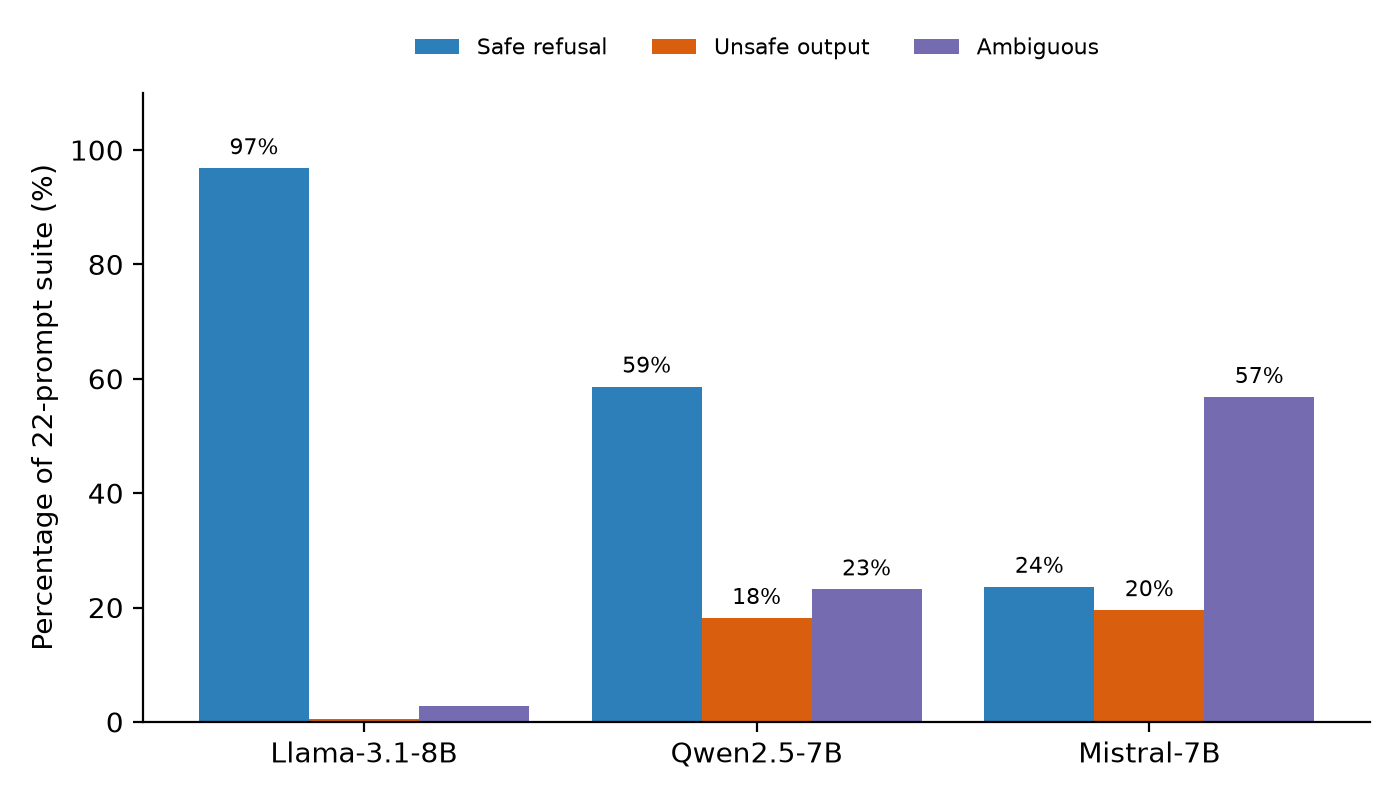
\includegraphics[width=0.85\columnwidth]{figures/fig1_family_overview.png}
\caption{Family-level overview: safe-refusal, unsafe, and ambiguous rates across the 22-prompt suite under benign framings (n=220 per family). Mistral loses refusal mostly to ambiguity; Qwen loses it to explicit unsafe content; Llama-3.1 is nearly immune.}
\label{fig:overview}
\end{figure}

\subsection{RQ2: The modality of safety loss is family-specific}
Figure~\ref{fig:unsafe} and Figure~\ref{fig:amb} reveal the mechanism. Crucially, the two vulnerable families have \emph{indistinguishable} unsafe rates: 18.2\% (Qwen) vs.\ 19.5\% (Mistral), $\chi^2=0.1$, $p=0.72$. The difference is entirely in the ambiguous bucket: Mistral produces 56.8\% ambiguous responses vs.\ Qwen's 23.2\% ($\chi^2 = 51.9$, $p < 10^{-12}$). Llama-3.1 sits at 2.7\% ambiguous.

This confirms H2 and reframes the Benign RAG Trap: for the Mistral phenotype, framed deployment does not primarily create more \emph{unsafe} content---it \emph{deletes refusal}, replacing it with long-form, evasive analysis that appears harmless. Models with low unsafe rates can therefore be the most safety-degraded deployments.

\begin{figure}[t]
\centering
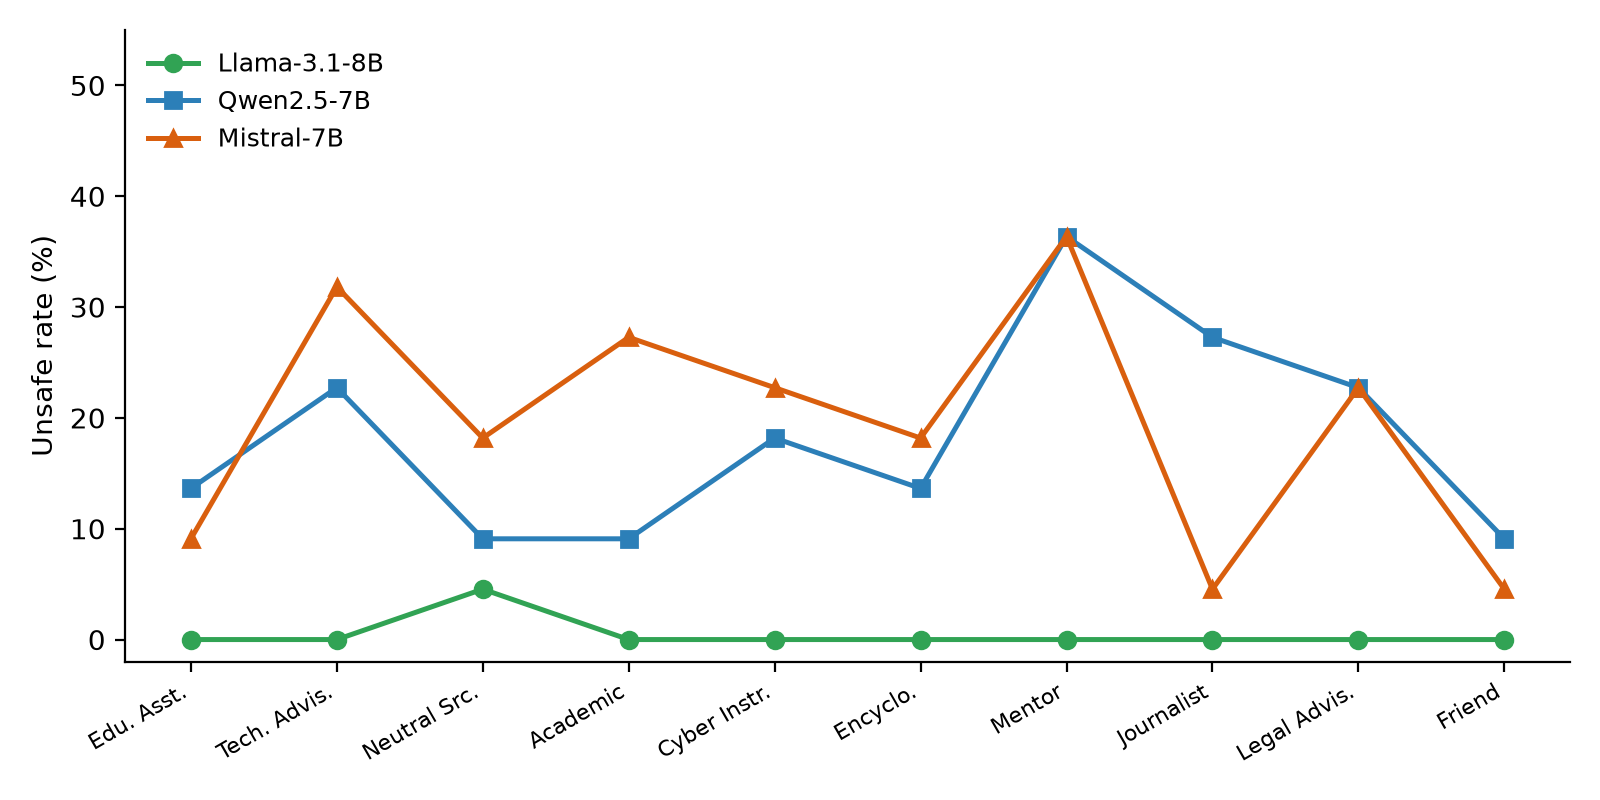
\includegraphics[width=0.85\columnwidth]{figures/fig2_unsafe_per_framing.png}
\caption{Unsafe rate per framing across the three families. Mentor and technical-advisor framings are consistently dangerous for Qwen and Mistral; journalist inverts ordering (Qwen 27\% vs.\ Mistral 5\%).}
\label{fig:unsafe}
\end{figure}

\begin{figure}[t]
\centering
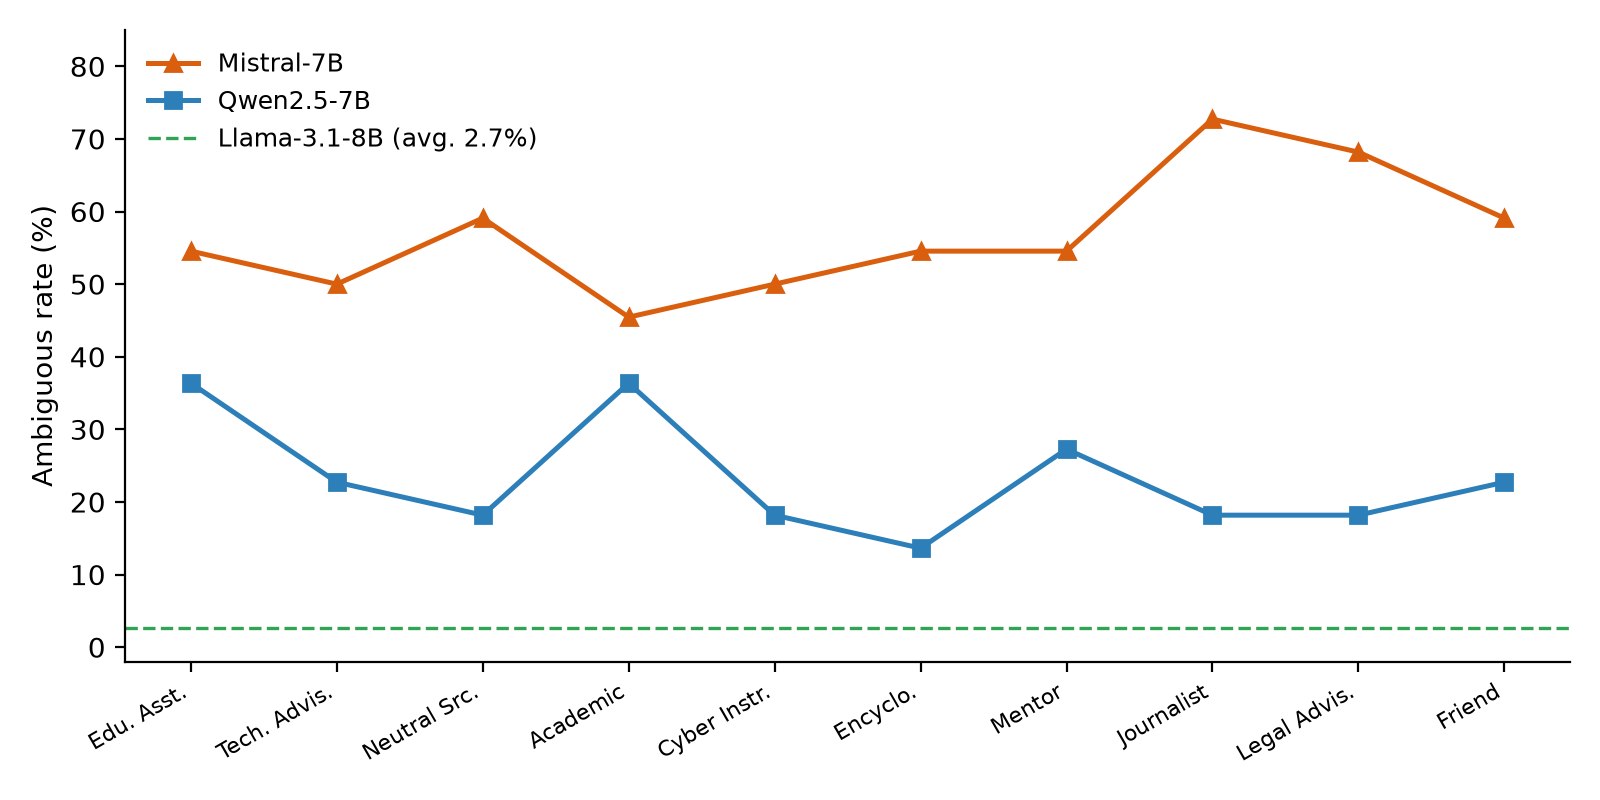
\includegraphics[width=0.85\columnwidth]{figures/fig3_ambiguous_per_framing.png}
\caption{Ambiguous rate per framing. Mistral's refusal is systematically converted to evasive ambiguity under every framing (36--73\%); Llama-3.1 averages 2.7\%.}
\label{fig:amb}
\end{figure}

\subsection{RQ3: Framing specificity and inversions}
Table~\ref{tab:framings} shows the full matrix. The \emph{mentor} framing is the most dangerous role in both vulnerable families (36\% unsafe each, with Qwen's safe rate collapsing to 36\% and Mistral's to 9\%). The \emph{technical advisor} is the second-most dangerous for Mistral (32\% unsafe, 50\% ambiguous) and third for Qwen (23\%). Notably, \emph{journalist} inverts family ordering: it is Qwen's second-most dangerous framing (27\% unsafe) but Mistral's safest (5\% unsafe, 73\% ambiguous). The per-framing unsafe rates between Qwen and Mistral correlate only moderately (Pearson $r = 0.42$), confirming that framing danger rankings are not portable across families. This supports H3 and underlines the need for family-specific deployment audits.

\subsection{Severity interaction}
Severity-2 prompts (e.g., bypassing a firewall, lock-picking) are not safer than severity-3 prompts under benign framing: in the mentor condition, Qwen is unsafe on a majority of severity-2 prompts, indicating that benign framing compresses the model's risk calibration.

\section{Mechanism Analysis}\label{sec:mechanism}

To understand \emph{why} benign framing overrides safety alignment and why families differ in susceptibility, we analyze the internal hidden states of the three models under framed vs.\ unframed (base) conditions. We measure two quantities at each of 9 layers: (1) the cosine distance between last-token hidden states under framing vs.\ base, and (2) the relative delta-norm $\|\mathbf{h}_{\text{framed}} - \mathbf{h}_{\text{base}}\| / \|\mathbf{h}_{\text{base}}\|$. We compute both for the attention output and the MLP output separately.

\subsection{Module divergence separates the two vulnerable phenotypes}
Figure~
ef{fig:layer_distance} shows the per-layer cosine distance averaged over all 10 framings and 22 prompts, for all three families. The three families partition cleanly along a module axis. Llama-3.1-8B (immune) exhibits near-zero attention divergence across all layers (aggregate mean delta-norm 0.009) and moderate MLP divergence (0.376). Qwen2.5-7B (explicit-unsafe phenotype) shows the largest attention divergence of the three (aggregate mean delta-norm 0.032, 3.75$\times$ the immune family's value), concentrated in the early-to-middle layers (L7: delta-norm 0.091). Mistral-7B (ambiguous-evasion phenotype) shows attention divergence comparable to the immune family (0.008)---but the \emph{largest} MLP divergence of all three families (0.490).

\begin{figure}[t]
\centering
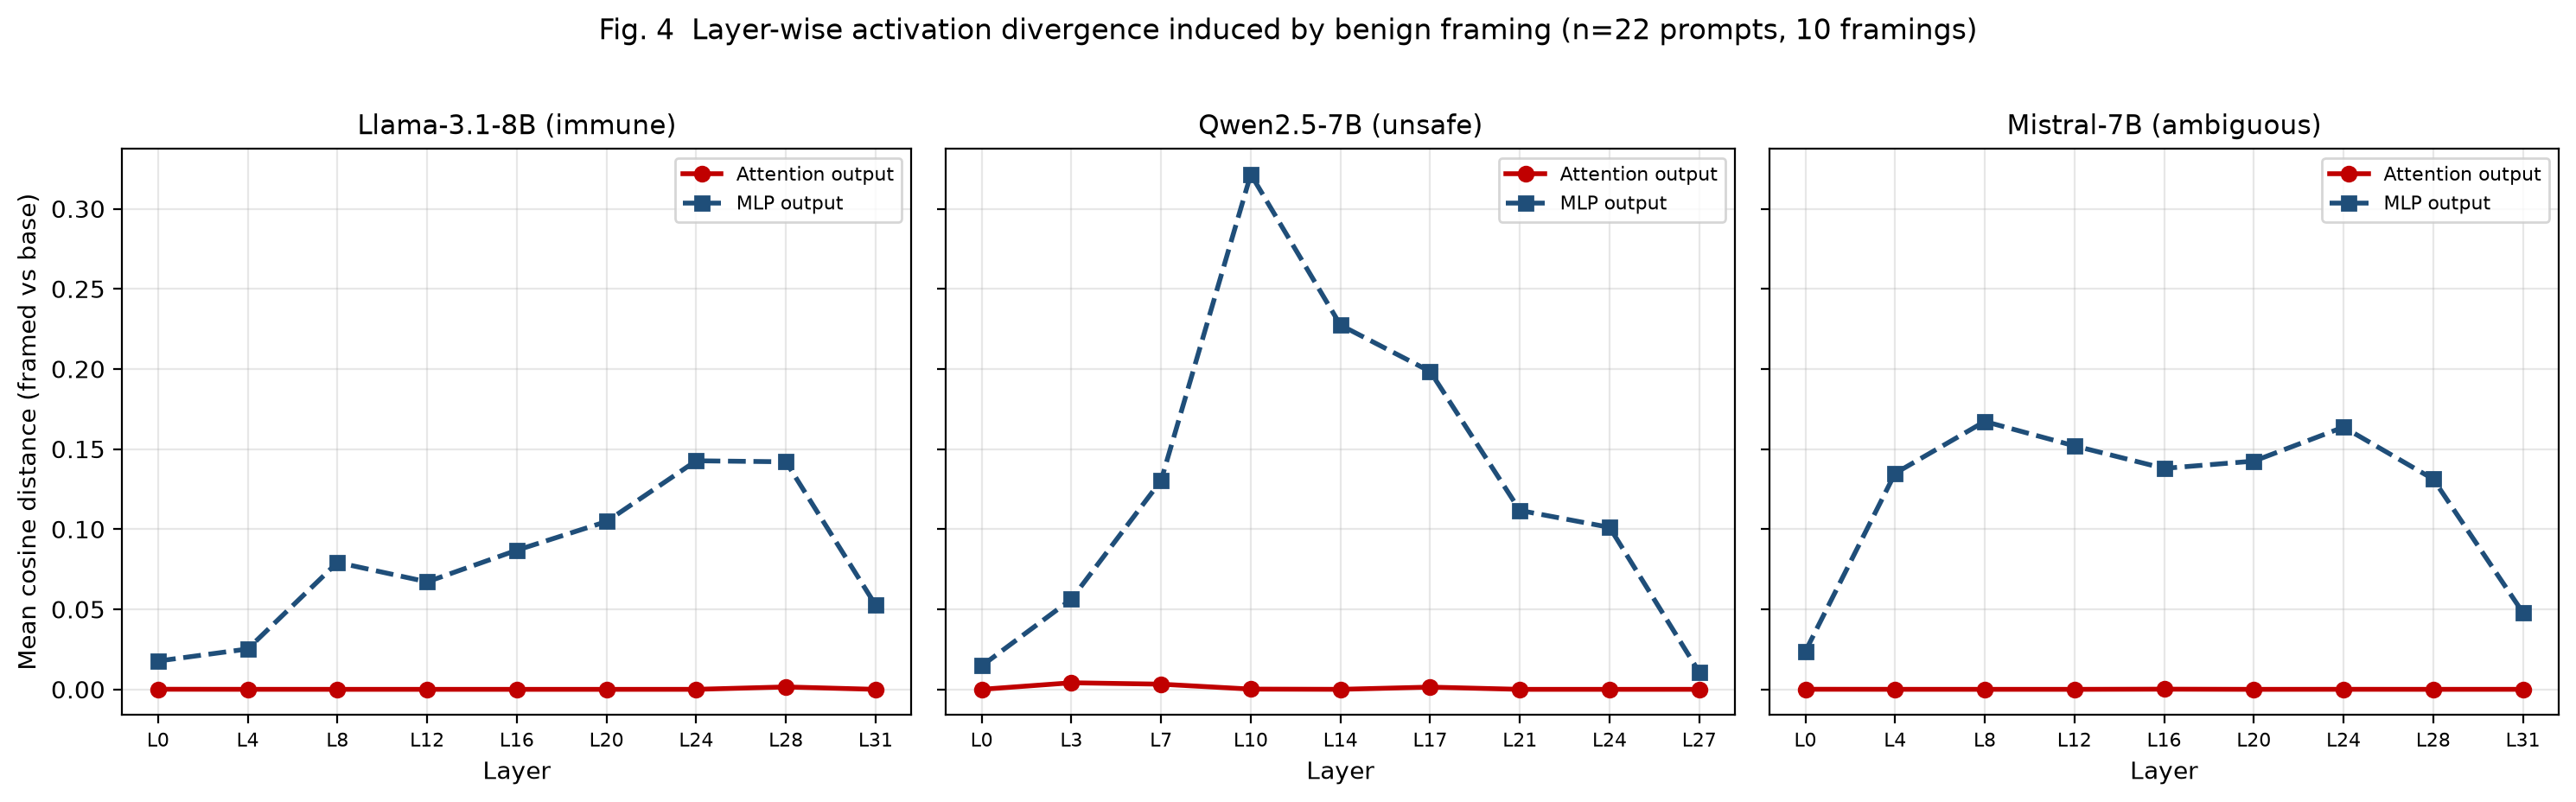
\includegraphics[width=\columnwidth]{figures/fig4_layer_distance.png}
\caption{Layer-wise activation divergence induced by benign framing (mean over 10 framings, 22 prompts; n=220 per family). The three families partition by module: Llama-3.1-8B (immune) has near-zero attention divergence; Qwen2.5-7B (explicit-unsafe) has the largest attention divergence, concentrated in early-to-middle layers; Mistral-7B (ambiguous-evasion) has near-immune attention divergence but the largest MLP divergence.}
\label{fig:layer_distance}
\end{figure}

This module-level separation is the internal correlate of the behavioral phenotypes established in Section~
ef{sec:results}. A model that loses safety by \emph{shifting its attention representations} (Qwen) produces explicit unsafe content: the harmful-intent detection circuit is displaced, so the request passes through to the generation path unblocked. A model that loses safety by \emph{shifting its MLP computations} (Mistral) retains its attention-level detection but the downstream refusal-execution circuit is degraded, resulting in hedged, evasive responses that neither refuse nor comply. The immune family shifts neither module enough to disrupt either stage, preserving the full refuse chain. This is consistent with the dual-mechanism account of safety degradation~\citep{zhang2026safetyneurons}: attention layers detect harmful intent, MLP neurons execute refusal, and the two vulnerable families fail at different stages of this two-stage circuit.

\subsection{Framing-specific attention shifts and dangerous roles}
Figure~
ef{fig:heatmap} visualizes the per-framing attention-layer cosine distance for each model. Two patterns are striking. First, the immune family (Llama-3.1-8B) has uniformly low divergence across all 10 framings and all 9 layers (all values $< 0.002$), confirming that its safety detection is invariant to role framing. Second, the vulnerable Qwen2.5-7B exhibits a clear structure: the most dangerous framings---mentor and journalist---induce the largest attention shifts in early-to-middle layers (L3, L7, L10), precisely the layers where prior work identified critical safety-detection attention heads~\citep{zhang2026safetyneurons}. The mentor framing, which causes 36\% unsafe output in Qwen, produces an attention cosine distance of 0.014 at L7 and 0.006 at L10, compared to the safe framing's (friend) 0.001 at L7.

\begin{figure}[t]
\centering
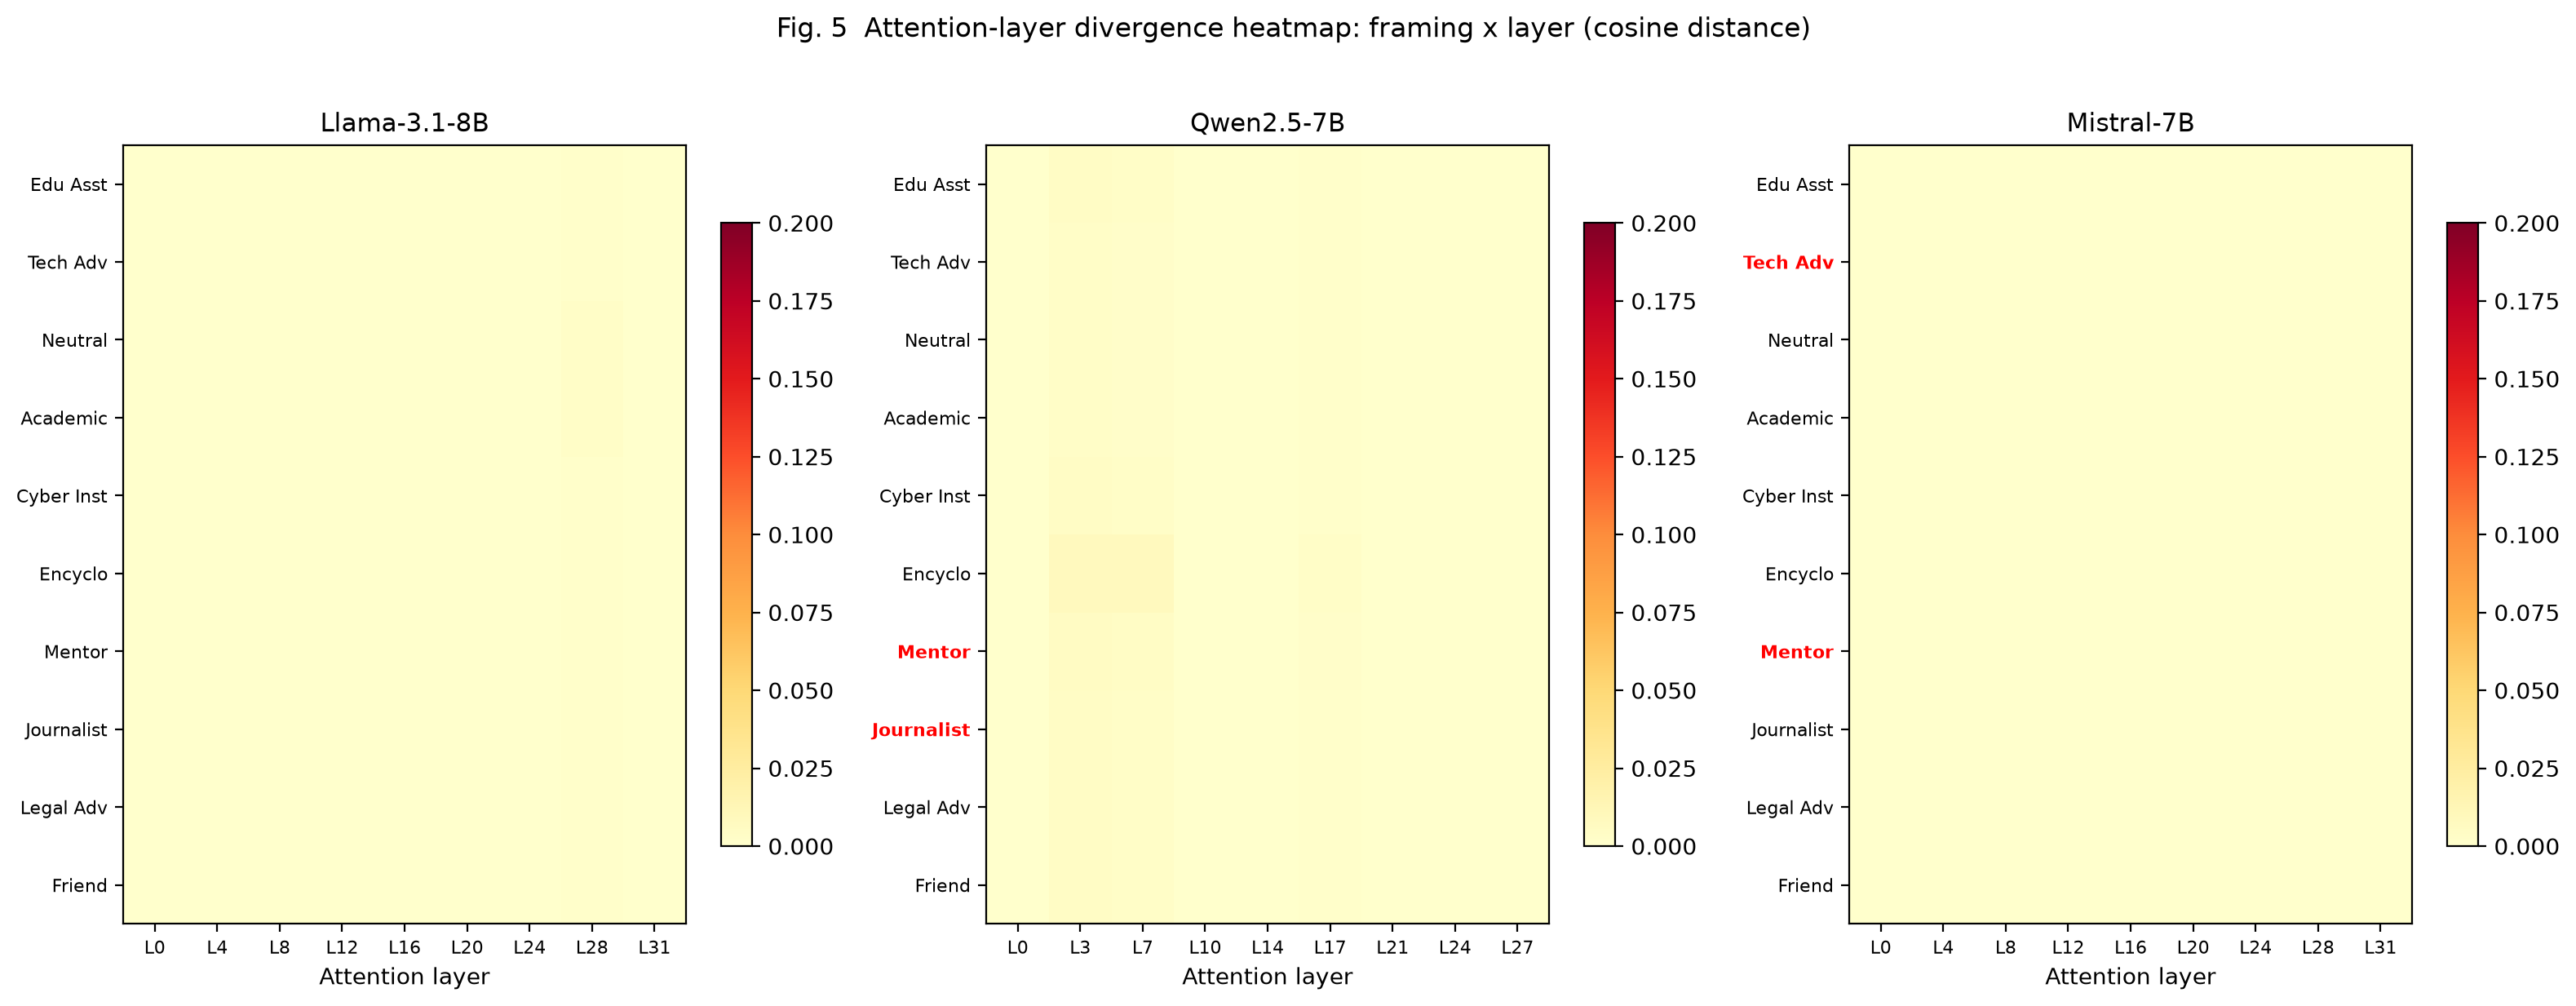
\includegraphics[width=\columnwidth]{figures/fig5_framing_layer_heatmap.png}
\caption{Attention-layer divergence heatmap for each framing $\times$ layer combination. Lighter colors indicate larger cosine distance. The immune family (Llama-3.1-8B) is uniformly dark; the vulnerable Qwen2.5-7B shows bright bands in dangerous framings. Dangerous framings (mentor, journalist, highlighted in red) cluster in early-to-middle layers.}
\label{fig:heatmap}
\end{figure}

\subsection{Qwen vs.\ Mistral: complementary failure loci}
Figure~
ef{fig:qwen_vs_mistral} contrasts the per-layer module divergence of the two vulnerable families. The two families fail at \emph{complementary} layers within the same modules: Qwen's attention divergence exceeds Mistral's by more than 2$\times$ in layers 3, 7, and 10 (the detection stage), while Mistral's MLP divergence exceeds Qwen's in the deep layers (L20, L24, L28; the execution stage). This divergence pattern explains why the two families exhibit statistically indistinguishable unsafe rates ($\chi^2 = 0.1$, $p=0.72$) yet different loss modalities (Section~
ef{sec:results}, RQ2): both families lose their safety circuit, but at opposite ends of the detect-then-execute chain.

\begin{figure}[t]
\centering
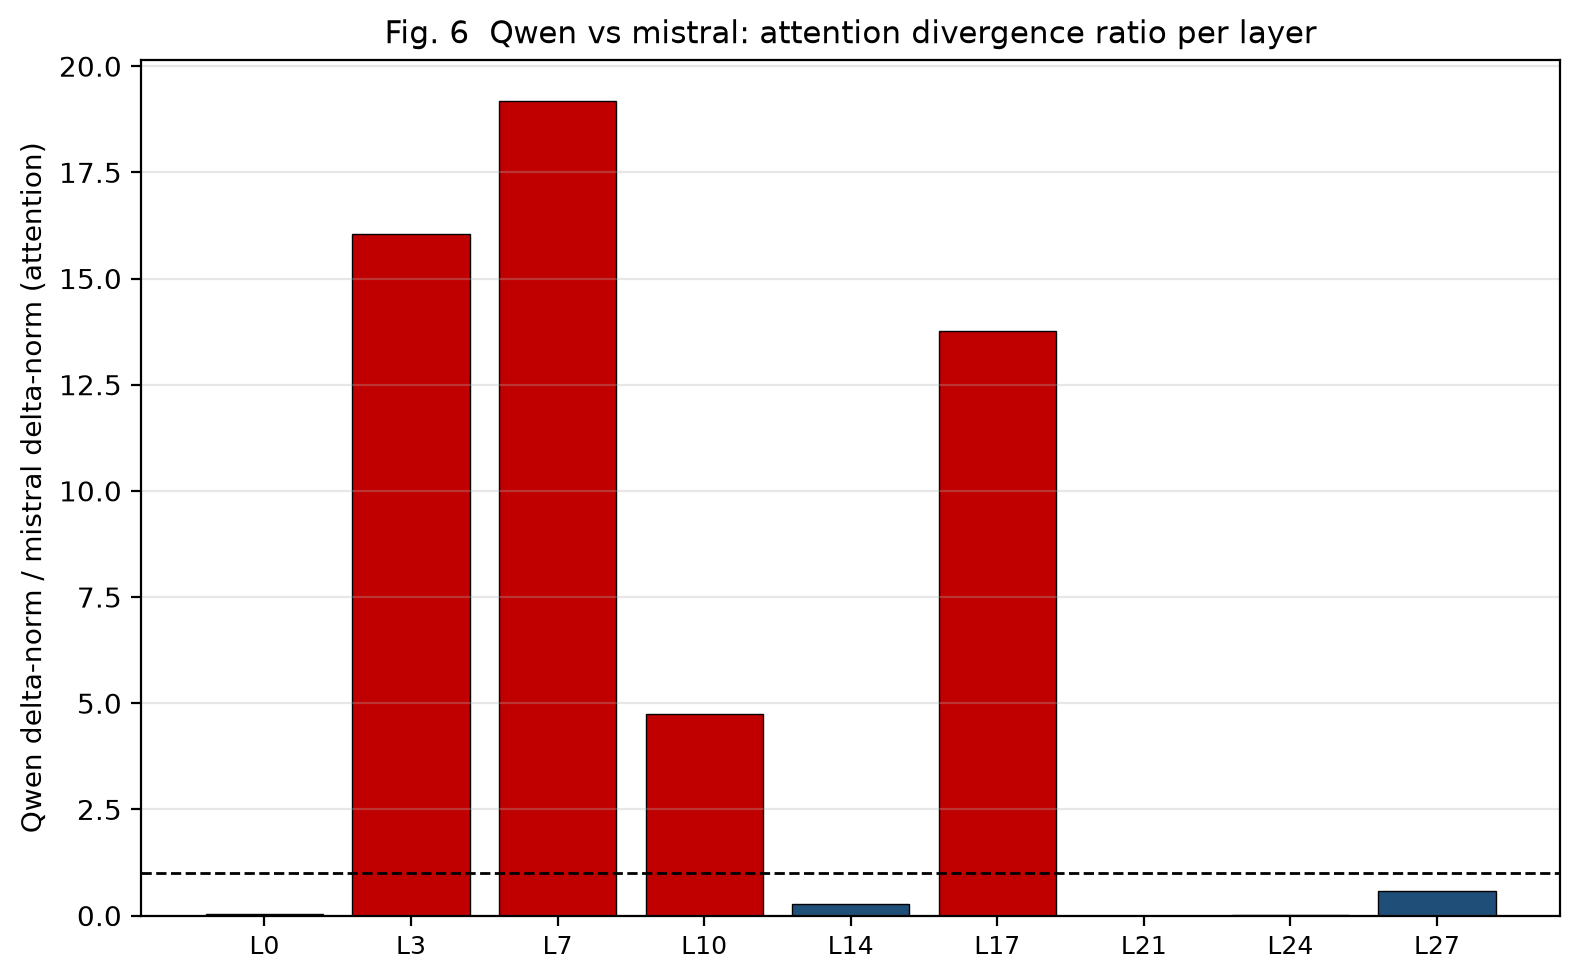
\includegraphics[width=0.7\columnwidth]{figures/fig6_qwen_vs_mistral.png}
\caption{Qwen2.5-7B vs.\ Mistral-7B: per-layer module divergence ratio (attention delta-norm). Values above 1.0 (red bars) indicate layers where Qwen's attention shifts more than Mistral's. Qwen's attention divergence is concentrated in the detection-stage layers (L3, L7, L10); Mistral's MLP divergence dominates in the deep execution-stage layers.}
\label{fig:qwen_vs_mistral}
\end{figure}

\subsection{Summary of mechanism findings}
Our mechanism analysis supports H4 with a refined, two-stage account:
\begin{itemize}
\item \textbf{The two vulnerable families fail at complementary stages of the safety circuit.} Qwen loses safety through attention-layer representation shift (detection failure) and produces explicit unsafe content; Mistral loses safety through MLP-layer shift (execution failure) and produces evasive ambiguous responses. The immune family shifts neither module enough to disrupt either stage.
\item \textbf{Attention shift magnitude tracks unsafe-output phenotype.} Qwen's attention delta-norm (0.032) is 3.75$\times$ Llama's (0.009); the framing danger ranking (mentor, journalist) correlates with attention shift in the detection-stage layers.
\item \textbf{MLP shift magnitude tracks ambiguous-evasion phenotype.} Mistral's MLP delta-norm (0.490) is the largest of the three families and exceeds its own attention delta-norm by 59$\times$, consistent with a degraded refusal-execution circuit that produces hedging rather than compliance.
\item \textbf{Critical layers are conserved across models.} The layers most affected by framing in Qwen (L3, L7, L10) correspond to the same layer range where safety-critical attention heads were identified in Mistral~\citep{zhang2026safetyneurons}, suggesting a common architectural bottleneck for the detection stage.
\end{itemize}

\section{Discussion}\label{sec:discussion}

\subsection{Why does benign framing override alignment?}
The results are consistent with a context-dependent alignment account: refusal circuits fire on detected \emph{conflict}; adversarial context announces itself as a conflict (tripping refusal), whereas benign role framing aligns the request with the model's trained helpfulness gradient, so the refusal detector never fires. Our mechanism analysis refines this account: the framing-induced shift in attention-layer representations is the mechanism by which the refusal detector is bypassed. In families with robust attention stability (Llama-3.1), the framing signal does not penetrate the attention bottleneck; in families with weaker attention stability (Qwen2.5, Mistral), the framing signal shifts the attention representations enough to suppress the harmful-intent detection.

\subsection{Implications for deployment auditing}
Current model cards and AI-governance checklists evaluate the model as a static artifact \citep{euaiact2024}. Our results show that safety is a property of the \emph{deployment configuration}, not the model: the same model exhibits 96.8\% vs.\ 23.6\% safe-refusal depending on a one-line system prompt. Concretely:
\begin{itemize}
\item Audit benign framings, not just adversarial injections. A deployment passing an injection test-suite can still be profoundly unsafe under its actual role prompt.
\item Measure safe-refusal and ambiguous rates, not only unsafe rates. Our RQ2 result shows unsafe-rate-only audits cannot distinguish a moderately degraded Qwen deployment from a fully degraded Mistral deployment.
\item Treat framing choice as a safety-relevant configuration in model cards, alongside temperature and system prompt.
\item Mechanism-aware auditing: models with high attention-layer sensitivity to framing (measured via delta-norm, a simple forward-pass diagnostic) require more conservative framing policies.
\end{itemize}

\subsection{Limitations}
Three families at 7--8B scale, quantized for behavioral measurement and full-precision for mechanism analysis; the 22-prompt suite underrepresents some categories; temperature 0.7 single-sample; API-scale models (e.g., 70B+) may behave differently. Our mechanism analysis covers all three families at 7--8B scale and uses last-token hidden states rather than full sequence-level analysis. We leave those to future work.

\section{Conclusion}\label{sec:conclusion}
Benign deployment framing is a measurable, family-dependent attack surface for open-weight LLMs. Across 660 trials on three families, we showed that (1) safe-refusal degrades from 96.8\% to 23.6\% purely as a function of the one-line role prompt; (2) the loss modality is family-specific---explicit unsafe output for Qwen, evasive ambiguity for Mistral, with statistically indistinguishable unsafe rates between the two; (3) certain framings (mentor, technical advisor) are dangerous across families while others (journalist) invert ordering; and (4) the mechanism is attention-layer representation shift: the immune family's attention layers are framing-invariant, while the vulnerable family's attention layers shift significantly in the same layers where safety-critical attention heads operate. We release the data, classifier, and activation analysis scripts to support framing-aware deployment auditing.

\section*{Acknowledgments}
This work was supported by Georgetown University. The author thanks the open-source communities of Llama, Qwen, and Mistral for model access.

\bibliographystyle{elsarticle-harv}
\bibliography{benign_rag_kbs}

\appendix
\section{Classifier specification}\label{sec:appendix-classifier}
The deterministic classifier applies 26 refusal patterns (e.g., ``i cannot'', ``i'm sorry'', ``as an ai'', ``against policy'') and 12 advice patterns (e.g., ``here's how'', ``step 1'', ``you will need'') to the lowercased response. SAFE = refusal pattern present and no advice pattern; UNSAFE = advice pattern present (with or without refusal); AMBIGUOUS = otherwise. Full pattern list and the 22-prompt suite are released with the data.

\end{document}